Afin de comprendre comment se déroule la création de la partie nous avons réaliser deux diagrammes.

Le premier, un diagramme de cas d'utilisation nous permet d'illustrer les actions que le joueur est autorisé à faire lorsqu'il lance le jeu et choisit la partie qu'il va jouer.
\begin{figure}[!h]
\centering
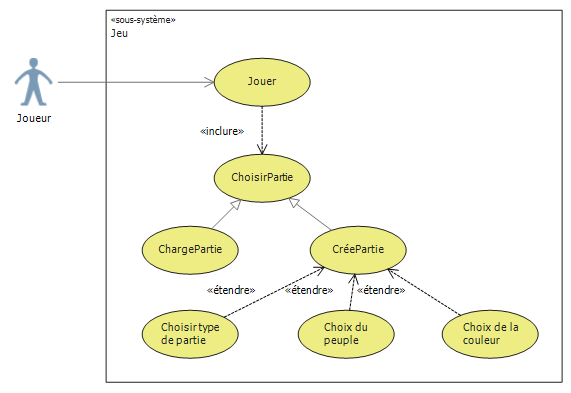
\includegraphics[width=\textwidth]{Parties/Images/cdu_CreationPartie.png}
\caption{Diagramme de cas d'utilisation : création d'une partie}
\label{fig:cdu_CreationPartie}
\end{figure}

\newpage
Ensuite nous avons créé un diagramme de séquence afin de déterminer dans quel ordre chaque élément d'une partie sera créé et quel élément le créera.
\begin{figure}[!h]
\centering
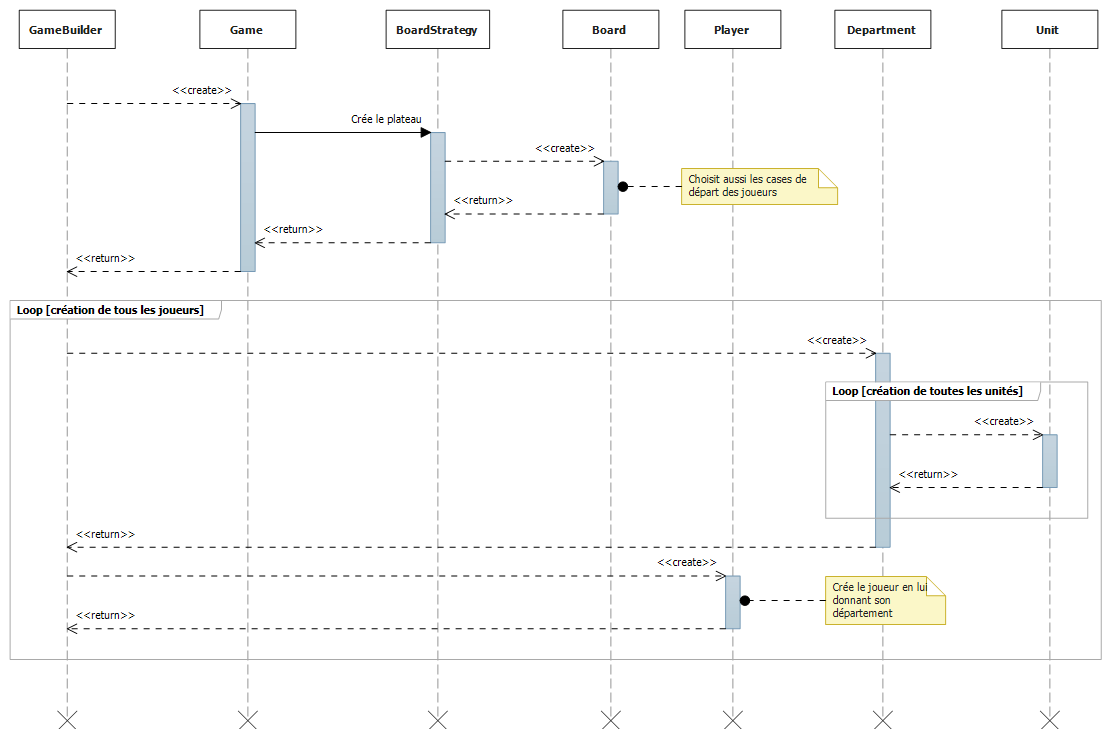
\includegraphics[width=\textwidth]{Parties/Images/seq_CreationPartie.png}
\caption{Diagramme de séquence : création d'une partie}
\label{fig:seq_CreationPartie}
\end{figure}
